\documentclass[border=0.8ex,svgnames,tikz]{standalone}
\usepackage{amsmath,mathtools}
\usepackage{fontspec}
\setmainfont{Source Serif 4}
\setsansfont{Source Sans 3}
\setmonofont{Source Code Pro}
\usetikzlibrary{chains}
\begin{document}
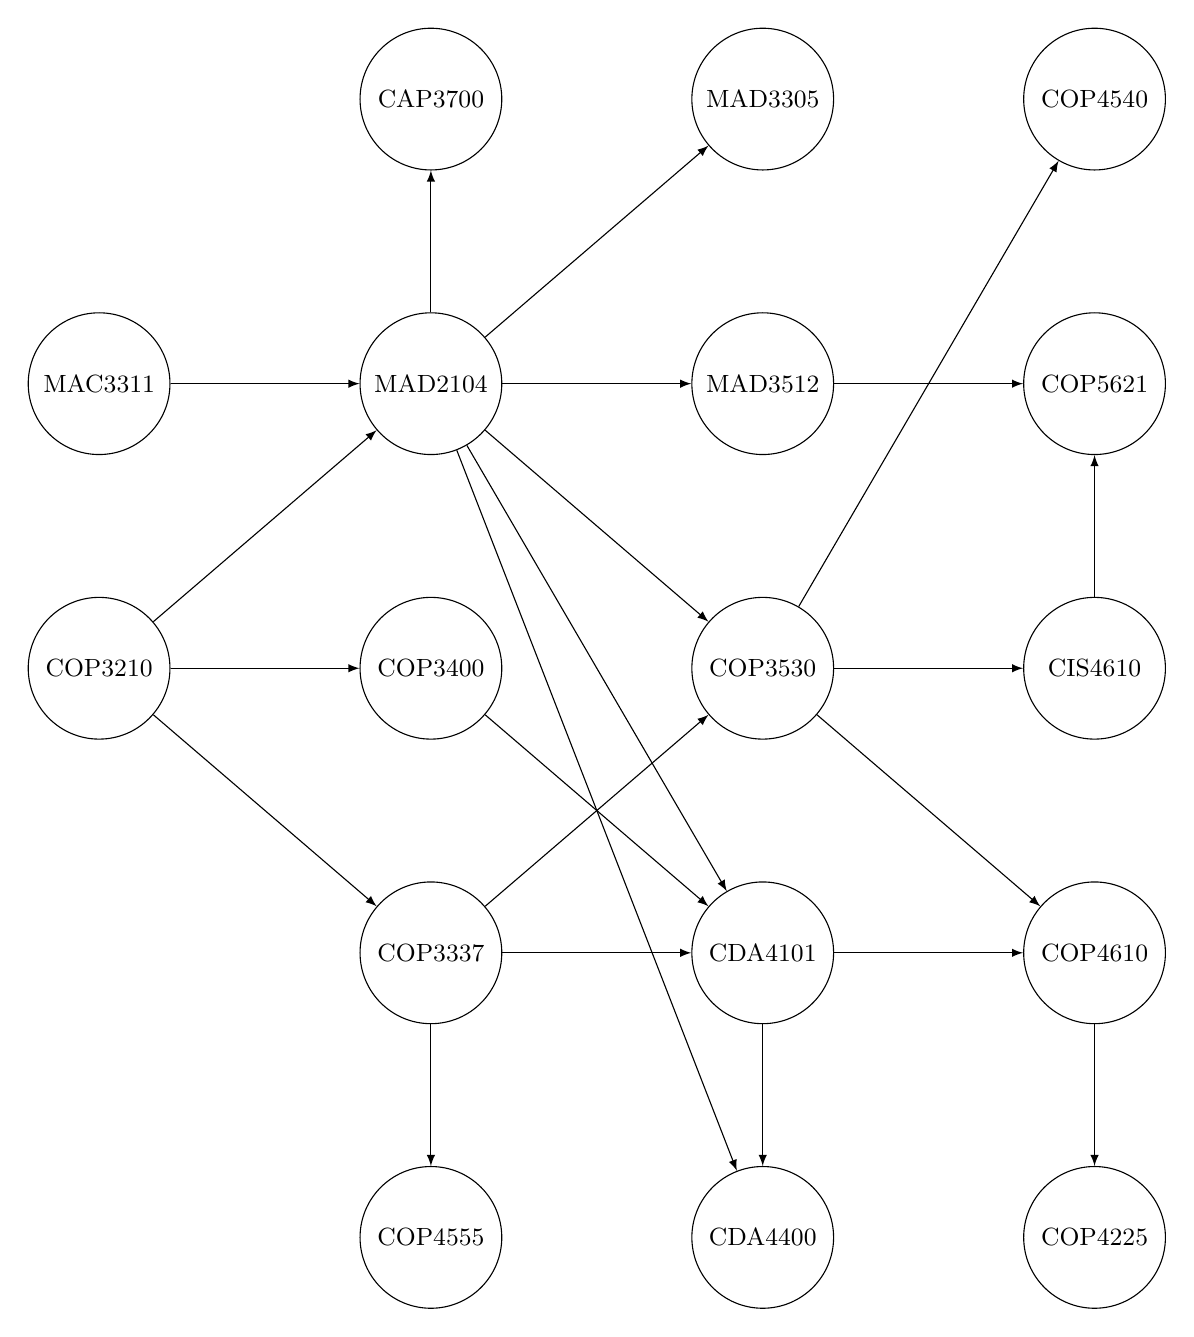
\begin{tikzpicture}[
  node distance=1.8cm and 2.4cm,
  every node/.style={draw,circle,minimum size=1.8cm,font=\small,on chain},
  empty node/.append style={draw=none,on chain},
  every path/.style={draw,>=latex},
  start chain=going below,
  ]
  \node[empty node](n11){};
  \node(n12){MAC3311};
  \node(n13){COP3210};
  \node[empty node](n14){};
  \node[empty node](n15){};
  \node[right=of n11](n21){CAP3700};
  \node(n22){MAD2104};
  \node(n23){COP3400};
  \node(n24){COP3337};
  \node(n25){COP4555};
  \node[right=of n21](n31){MAD3305};
  \node(n32){MAD3512};
  \node(n33){COP3530};
  \node(n34){CDA4101};
  \node(n35){CDA4400};
  \node[right=of n31](n41){COP4540};
  \node(n42){COP5621};
  \node(n43){CIS4610};
  \node(n44){COP4610};
  \node(n45){COP4225};
  \path[->]
  (n12) edge (n22)
  (n13) edge (n22)
  (n13) edge (n23)
  (n13) edge (n24)
  (n22) edge (n21)
  (n22) edge (n31)
  (n22) edge (n32)
  (n22) edge (n33)
  (n22) edge (n34)
  (n22) edge (n35)
  (n23) edge (n34)
  (n24) edge (n25)
  (n24) edge (n33)
  (n24) edge (n34)
  (n32) edge (n42)
  (n33) edge (n41)
  (n33) edge (n43)
  (n33) edge (n44)
  (n34) edge (n35)
  (n34) edge (n44)
  (n43) edge (n42)
  (n44) edge (n45);
\end{tikzpicture}
\end{document}
